\documentclass[aspectratio=169,10pt]{beamer}
\usetheme{Madrid}
\usecolortheme{default}
\setbeamertemplate{navigation symbols}{}

% ----- Linux Mint-inspired Colors -----
\definecolor{mintbg}{RGB}{46,52,54}
\definecolor{mintpanel}{RGB}{56,62,64}
\definecolor{mintbar}{RGB}{63,70,72}
\definecolor{mintgreen}{RGB}{135,192,107}
\definecolor{mintgreenlight}{RGB}{165,214,167}
\definecolor{textgray}{RGB}{236,239,241}
\definecolor{codebg}{RGB}{34,39,40}
\definecolor{codeframe}{RGB}{92,107,95}
\definecolor{codetext}{RGB}{232,245,233}
\definecolor{codekeyword}{RGB}{167,214,104}
\definecolor{codestring}{RGB}{255,204,128}
\definecolor{codecomment}{RGB}{144,164,174}

% ----- Global Beamer Colors -----
\setbeamercolor{background canvas}{bg=mintbg}
\setbeamercolor{normal text}{fg=textgray,bg=mintbg}
\setbeamercolor{structure}{fg=mintgreen}
\setbeamercolor{title}{fg=mintgreen,bg=mintbg}
\setbeamercolor{subtitle}{fg=mintgreenlight,bg=mintbg}
\setbeamercolor{frametitle}{fg=mintgreen,bg=mintbar}
\setbeamercolor{titlelike}{fg=mintgreen,bg=mintbg}
\setbeamercolor{author}{fg=textgray,bg=mintbg}
\setbeamercolor{institute}{fg=textgray,bg=mintbg}
\setbeamercolor{date}{fg=mintgreenlight,bg=mintbg}
\setbeamercolor{section in toc}{fg=mintgreen}
\setbeamercolor{subsection in toc}{fg=textgray}
\setbeamercolor{itemize item}{fg=mintgreen}
\setbeamercolor{itemize subitem}{fg=mintgreenlight}
\setbeamercolor{itemize subsubitem}{fg=mintgreenlight}
\setbeamercolor{block title}{fg=mintgreen,bg=mintpanel}
\setbeamercolor{block body}{fg=textgray,bg=mintpanel}
\setbeamercolor{palette primary}{fg=mintgreen,bg=mintbar}
\setbeamercolor{palette secondary}{fg=textgray,bg=mintpanel}
\setbeamercolor{palette tertiary}{fg=mintgreen,bg=mintbar}
\setbeamercolor{palette quaternary}{fg=textgray,bg=mintpanel}
\setbeamercolor{headline}{bg=mintbar,fg=mintgreen}
\setbeamercolor{footline}{bg=mintbar,fg=textgray}
\setbeamercolor{separation line}{bg=mintgreen}
\setbeamercolor{fine separation line}{bg=mintgreen}

% ----- Font Settings -----
\setbeamerfont{title}{family=\ttfamily,series=\bfseries,size=\Large}
\setbeamerfont{subtitle}{family=\ttfamily,size=\normalsize}
\setbeamerfont{frametitle}{family=\ttfamily,series=\bfseries,size=\large}
\setbeamerfont{titlelike}{family=\ttfamily,series=\bfseries}
\setbeamerfont{section title}{family=\ttfamily,series=\bfseries}
\setbeamerfont{author}{family=\ttfamily,size=\small}
\setbeamerfont{institute}{family=\ttfamily,size=\small}
\setbeamerfont{date}{family=\ttfamily,size=\small}

% ----- Visible Itemize Markers -----
\setbeamertemplate{itemize item}{\color{mintgreen}\large\textbullet}
\setbeamertemplate{itemize subitem}{\color{mintgreenlight}\normalsize\textbullet}
\setbeamertemplate{itemize subsubitem}{\color{mintgreenlight}\small\textbullet}
\newcommand{\gitem}{\item[\textcolor{mintgreen}{\large\textbullet}]}

% ----- Terminal-style Frame Titles -----
\setbeamertemplate{frametitle}{%
  \nointerlineskip
  \begin{beamercolorbox}[wd=\paperwidth,ht=3.1ex,dp=1.1ex,leftskip=0.8em,rightskip=0.3em]{frametitle}
    {\usebeamerfont{frametitle}\textcolor{mintgreen}{>}\hspace{0.4em}\insertframetitle}
  \end{beamercolorbox}%
}

% ----- Rounded Madrid-like Title Page -----
\setbeamertemplate{title page}{%
  \vfill
  \begin{center}
    \begin{beamercolorbox}[wd=0.88\paperwidth,rounded=true,shadow=true,sep=1.51em,left]{block title}
      {\usebeamerfont{title}\textcolor{mintgreen}{>}\hspace{0.5em}\inserttitle\par}
      \vspace{0.4em}
      {\usebeamerfont{subtitle}\insertsubtitle\par}
    \end{beamercolorbox}
    \vspace{1.4em}
    {\usebeamerfont{author}\insertauthor\par}
    \vspace{0.5em}
    {\usebeamerfont{institute}\insertinstitute\par}
    \vspace{0.5em}
    {\usebeamerfont{date}\insertdate\par}
  \end{center}
  \vfill
}

\AtBeginSection[]{
\begin{frame}[plain]
  \vfill
  \centering
  {\usebeamerfont{title}\textcolor{mintgreen}{>}\hspace{0.35em}\insertsection\par}
  \vspace{0.6cm}
  {\ttfamily\color{textgray}loading module...}
  \vfill
\end{frame}
}

% ----- Packages -----
\usepackage[T1]{fontenc}
\usepackage[utf8]{inputenc}
\usepackage{hyperref}
\usepackage{graphicx}
\usepackage{minted}
\usepackage{tikz}
\usepackage{pgfplots}
\pgfplotsset{compat=1.18}
\usepackage{booktabs}
\usepackage{amsmath}
\usepackage{amssymb}
\usepackage{float}
\usepackage{enumitem}
\usepackage{tikz}
\usetikzlibrary{arrows.meta,positioning}
\usepackage{float}
\usepackage{svg}

% ----- Minted Style -----
\usemintedstyle{native}
\setminted{
  fontsize=\small,
  bgcolor=codebg,
  linenos,
  breaklines,
  framesep=2mm,
  tabsize=2,
  style=native
}

% ----- Title Page -----
\title[Hardening Email Sender Authentication]{Hardening Email Sender Authentication: \\ A Lab-Based Evaluation of SPF/DKIM/DMARC Misconfigurations}
\author[Guilherme, Jo\~ao, Ayrton, Ana]{Guilherme Ferreira \and Jo\~ao Oliveira \and Ayrton da Cruz \and Ana L\'ucia Ferreira}
\institute[FEUP]{Faculdade de Engenharia -- Universidade do Porto}
\date{\today}

% ----- Begin Document -----
\begin{document}

\begin{frame}[plain]
  \titlepage
\end{frame}

\begin{frame}{Table of Contents}
  \transdissolve
  \tableofcontents
\end{frame}

% ======================
\section{Introduction}
% ======================
\subsection{Why Email Spoofing Still Works}
\begin{frame}{Why Email Spoofing Still Works}
  \transdissolve
  \begin{block}{>> Problem}
      \begin{itemize}
        \item Phishing campaigns still succeed because email sender authentication is often misconfigured or only partially deployed.
        \item Attackers can impersonate trusted identities even when some authentication mechanisms seem to be enabled.
      \end{itemize} 
      \vspace{10pt}
   \end{block}
   \vfill
   \begin{block}{>> Project Goal}
      \begin{itemize}
        \item Build a controlled lab to reproduce spoofing attacks.
        \item Systematically analyze how SPF, DKIM and DMARC misconfigurations affect spoofing success and how to fix them.
      \end{itemize}
      \vspace{10pt}
    \end{block}
\end{frame}

\subsection{Research Questions \& Contributions}
\begin{frame}{Research Questions \& Contributions}
  \transdissolve
  \begin{block}{>> Preliminary Studies}
        \begin{itemize}
            \item Under which SPF, DKIM and DMARC configurations does spoofing still succeed?
            \item How do protocol composition flaws (e.g., relaxed alignment, parser inconsistencies) impact authentication?
            \item Can SMTP artefacts be used to detect spoofed emails automatically?
        \end{itemize}
    \end{block}
    \vspace{0.4cm}
    \begin{block}{>> Development Contributions}
        \begin{itemize}
            \item Docker-based lab for sender-authentication experiments.
            \item Systematic exploration of SPF/DKIM/DMARC misconfigurations.
            \item Evaluation of infrastructure hardening and ML-based detection.
        \end{itemize}
    \end{block}
\end{frame}

\subsection{Experimental Workflow}
\begin{frame}{Experimental Workflow}
  \transdissolve
  \begin{columns}[T]
    \column{0.5\textwidth}
    \begin{block}{>> Project Development}
      \begin{itemize}
        \item Infrastructure setup: Docker, BIND, Postfix/Dovecot, webmail.
        \item Authentication baseline: SPF, DKIM, DMARC behaviour.
        \item Spoofing attacks: \texttt{swaks}, \texttt{espoofer}, custom scripts.
        \item SMTP artefact collection: logs, headers, authentication traces.
        \item Feature extraction and ML-based spoofing detection.
        \item Infrastructure hardening and re-evaluation.
      \end{itemize}
    \end{block}
    \column{0.49\textwidth}
	  	\vspace{-20pt}      
      	\centering
        \begin{figure}
            \centering
            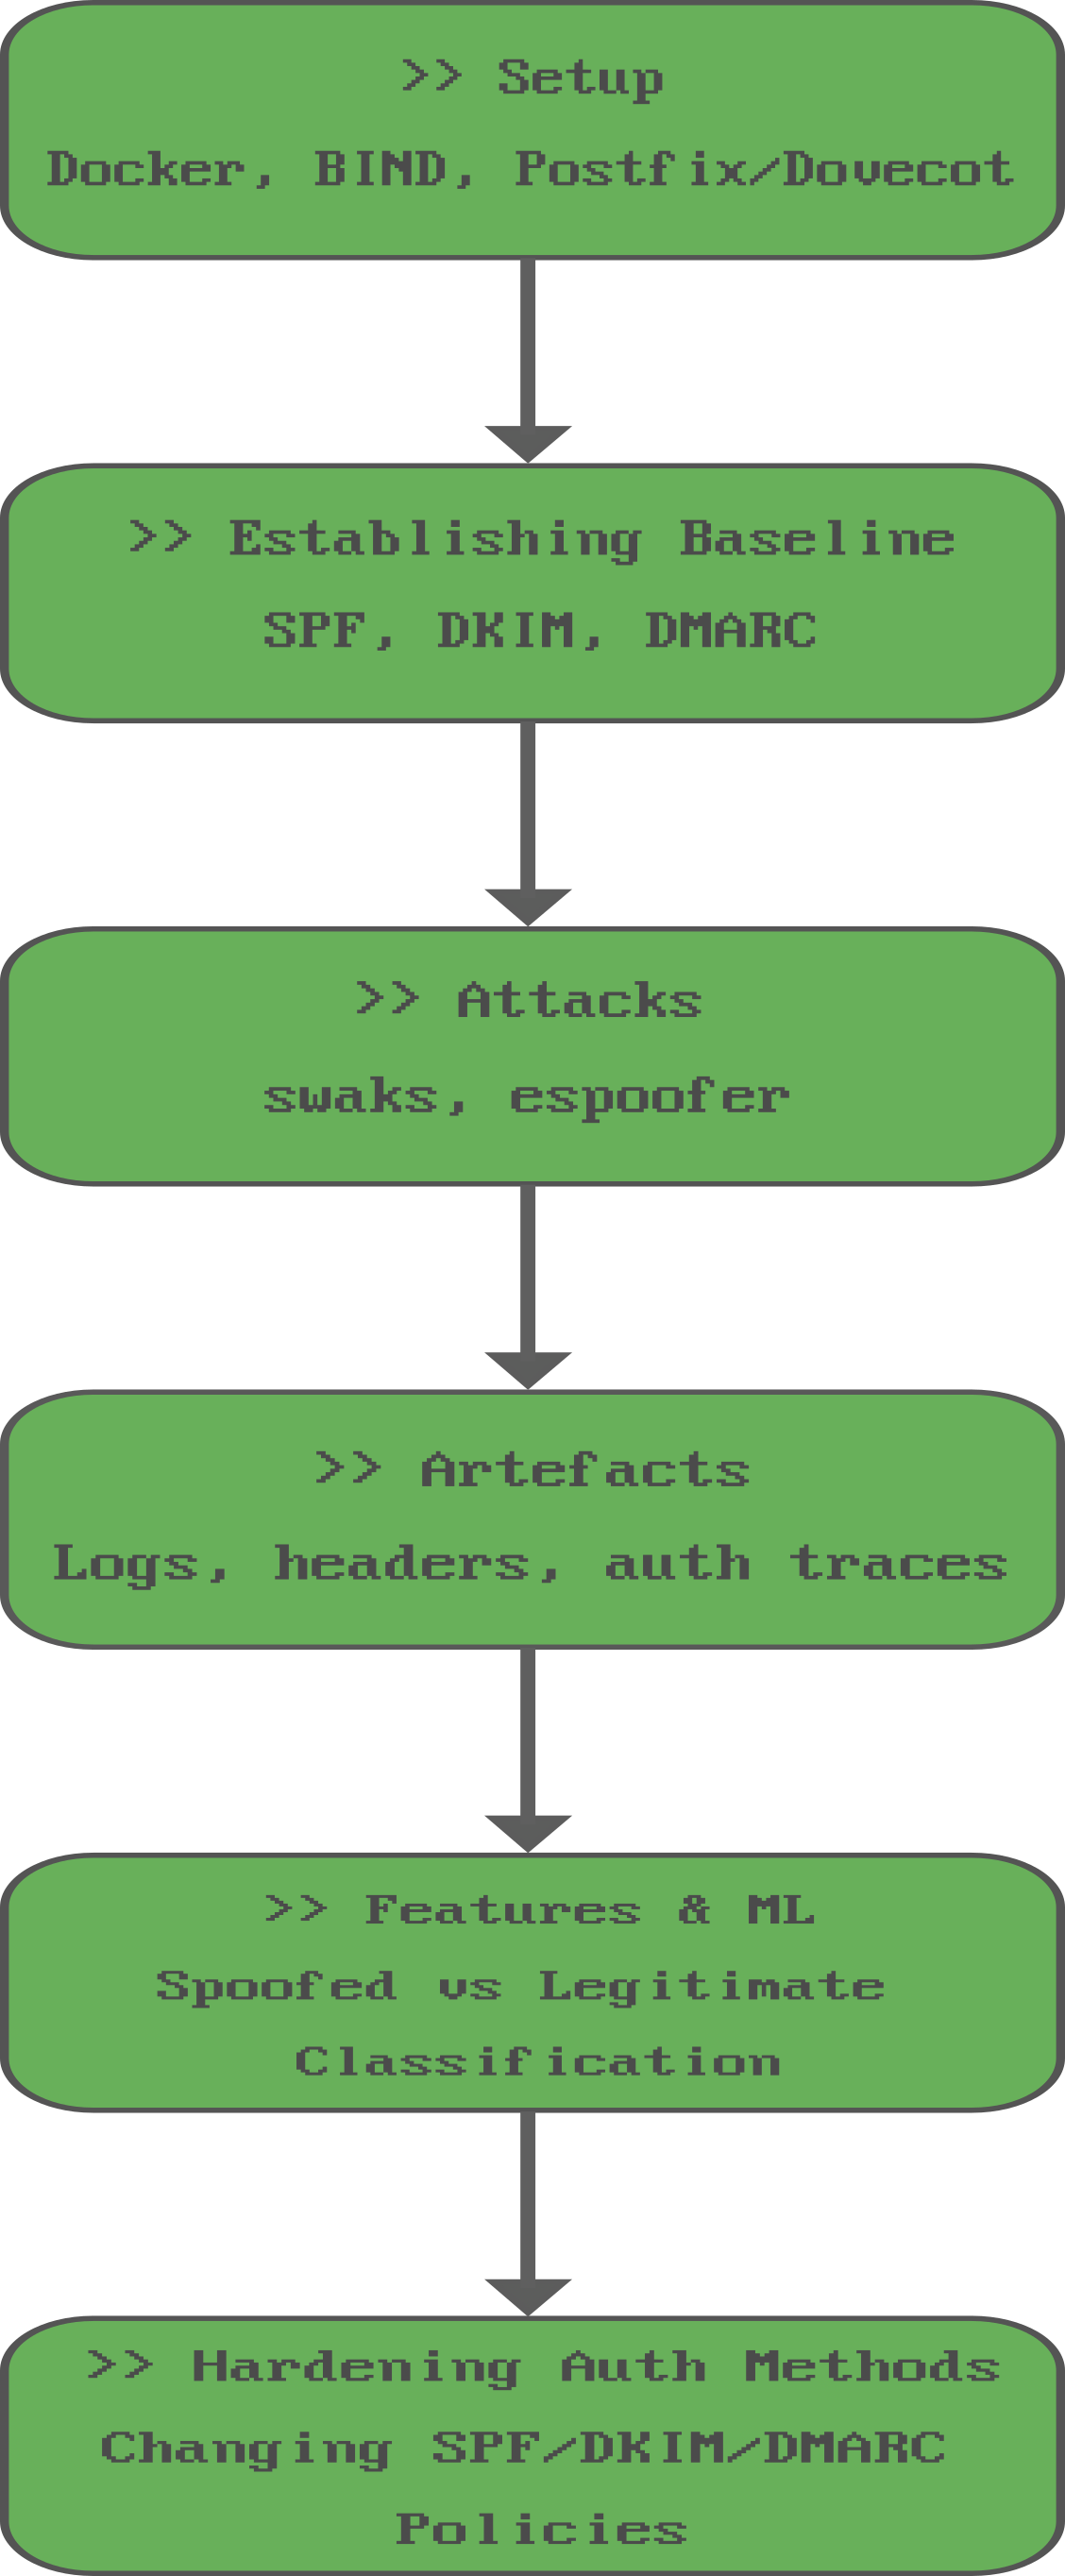
\includegraphics[width=0.4\linewidth]{workflow.png}
        \end{figure}
  \end{columns}
\end{frame}

\subsection{Development Highlighs}
\begin{frame}[fragile]{Development Highlights}
  \transdissolve
  \begin{block}{>> \texttt{SpoofMaster}}
  	\begin{itemize}
   	 	\item Helper tool to orchestrate spoofing tests inside the lab.
    		\item Wraps \texttt{attack.sh} script using \texttt{swaks} - aka. Swiss Army Knife.
    		\item Produces artefacts later used for ML-based detection.
  	\end{itemize}
  \end{block}
  \vfill
  \begin{minted}{bash}
   _____  ___    ___   ___  ____  __  __  ___   _____ ______________ ____
  / ____||  _ \ / _ \ / _ \| ___||  \/  |/ _ \ / ____|_   __|  ____||  _ \
 | (___  | |_) | | | | | | | |_  | \  / | /_\ \| (___   | | | |__   | |_) |
  \___ \ |  _ /| | | | | | |  _| | |\/| |/___\ \____ \  | | |  __|  |    /
  ____) || |   | |_| | |_| | |   | |  | |     \ \___) | | | | |____ | |\ \
 |_____/ |_|    \___/ \___/|_|   |_|  |_|      \_\____/ |_| |______||_| \_\

  ** Welcome to SpoofMaster – SPF/DKIM/DMARC Bypass Demo - SEED Labs **  
  \end{minted}
\end{frame}

\subsection{Lab Architecture}
\begin{frame}{Lab Architecture}
  \transdissolve
  \begin{columns}[T]
    \column{0.55\textwidth}
      \begin{block}{>> Lab Docker Network Setup}
      \begin{itemize}
        \item Isolated Docker network with four main containers:
        \begin{itemize}
          \item DNS server (BIND) hosting SPF/DKIM/DMARC records.
          \item Victim mail server (Postfix + Dovecot).
          \item Attacker container running \texttt{swaks} and Espoofer.
          \item Webmail client for victim-side inspection.
        \end{itemize}
        \item No connectivity to the real Internet to keep attacks contained.
      \end{itemize}
    \end{block}
    \column{0.45\textwidth}
      \begin{figure}
        \centering
        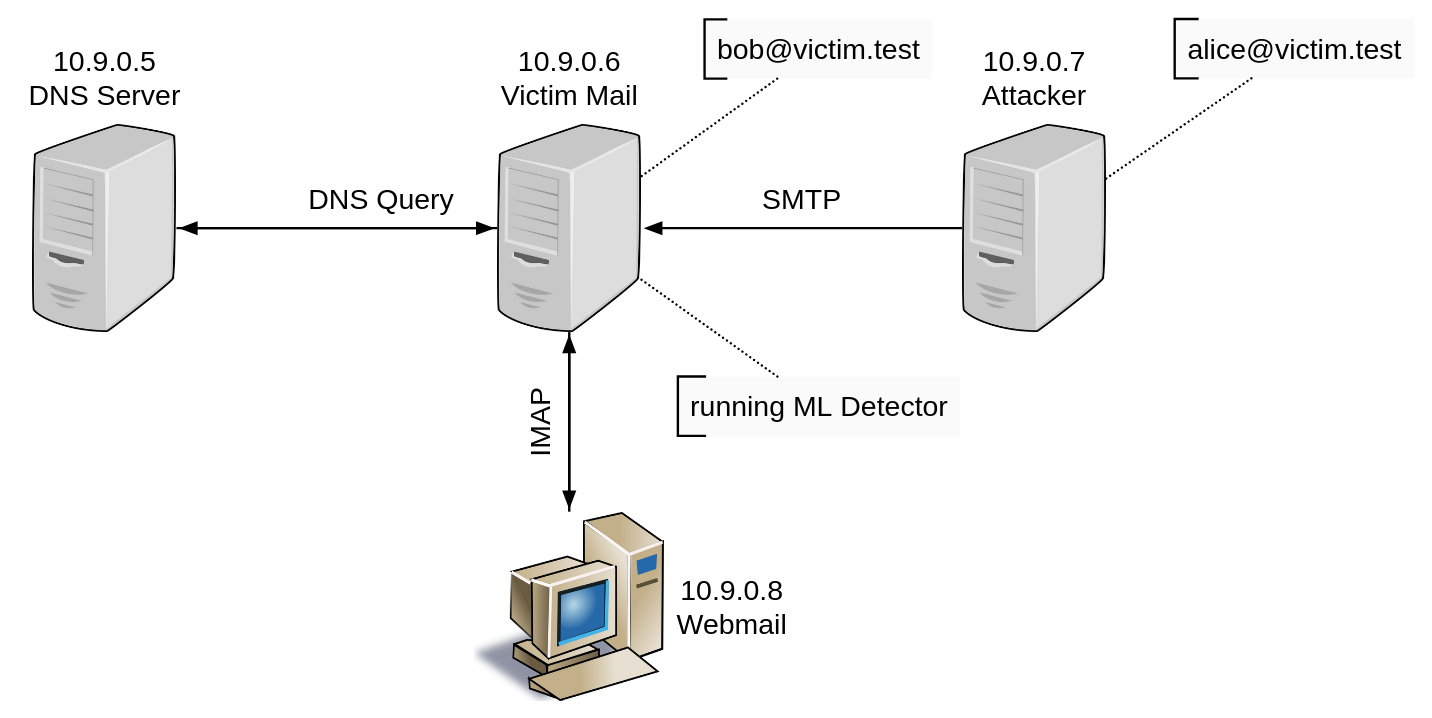
\includegraphics[width=0.95\linewidth]{networkdiagram.png}
        \caption{Docker-based isolated mail infrastructure}
      \end{figure}
  \end{columns}
\end{frame}

% =========================
\section{Authentication Protocols}
% =========================
\subsection{SPF, DKIM and DMARC}
\begin{frame}{SPF, DKIM and DMARC Overview}
  \transdissolve
  \begin{block}{>> Roles} 
  \begin{itemize}
    \item SPF validates the sending IP against the domain in the SMTP envelope (\texttt{MAIL FROM}).
    \item DKIM attaches a cryptographic signature that covers selected headers and body.
    \item DMARC combines SPF/DKIM results and enforces domain alignment and policy. 
  \end{itemize} \vspace{10pt}
  \end{block}
  \vfill
  \begin{block}{>> Insight}
  \begin{itemize}
    \item Authentication does not automatically mean security: misconfiguration or weak policies can still allow spoofed messages to be delivered.
  \end{itemize} \vspace{10pt}
  \end{block}
\end{frame}

\subsection{Potential Misconfigurations}
\begin{frame}[fragile]{Where Misconfigurations Appear}
  \transdissolve
  \begin{columns}[T]
    \column{0.40\textwidth}
      \begin{block}{>> Examples from the Lab}
      \begin{itemize}
        \item SPF: \verb|v=spf1 mx ~all| (soft-fail, accepts suspicious senders).
        \item DKIM: selector not published or key mismatch.
        \item DMARC: \verb|v=DMARC1; p=none; aspf=r; adkim=r| (monitoring only, relaxed alignment).
      \end{itemize}
      \end{block}
    \column{0.60\textwidth}
    \vspace{5pt}
    	\begin{figure}[H]
      \centering
      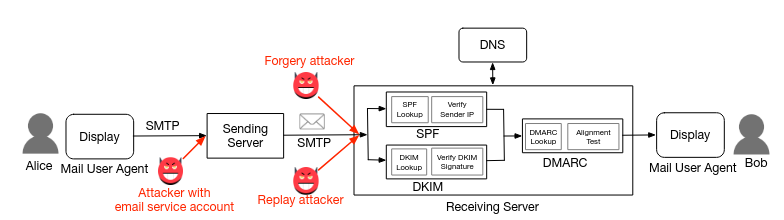
\includegraphics[width=\textwidth]{misconfiguration_highlights.png}
      \caption{Image from Chen et al. 2020}
    \end{figure}
    \begin{block}{>> Impact}
      \begin{itemize}
        \item Suspicious mail is accepted or only logged.
        \item Spoofed visible identities are not blocked.
      \end{itemize}
     \end{block}
  \end{columns}
\end{frame}

% ====================
\section{Spoofing Attacks}
% ====================

\subsection{Spoofing with SPF only}
\begin{frame}[fragile]{SPF-Based Spoofing Scenario}
  \transdissolve
  \begin{block}{>> Setup}
  \begin{itemize}
    \item SPF configured with soft-fail (\verb|~all|) and permissive host entries.
    \item Attacker sends mail using \texttt{swaks} with:
      \begin{itemize}
        \item Envelope sender: \texttt{attacker@attacker.test}.
        \item Visible \texttt{From:} header: \texttt{Alice <alice@victim.test>}.
      \end{itemize} \vspace{10pt}
  \end{itemize}
  \end{block}
  \vfill
  \begin{block}{>> Observation}
  \begin{itemize}
    \item SPF can pass because the envelope sender is allowed.
    \item The user still sees a spoofed identity in the visible \texttt{From} header.
  \end{itemize} \vspace{10pt}
  \end{block}
\end{frame}

\subsection{Open Source Email Spoofer Tool}
\begin{frame}{Advanced Authentication Bypass (\texttt{espoofer})}
  \transdissolve
  \begin{block}{>> Attack Goal}
  \begin{itemize}
    \item Exploit composition flaws and parser inconsistencies to bypass SPF, DKIM and DMARC simultaneously.
  \end{itemize}
  \end{block}
  \vfill
  \begin{block}{>> Techniques}
  \begin{itemize}
    \item Carefully crafting multiple \texttt{From} headers.
    \item Taking advantage of relaxed alignment and inconsistent header parsing.
    \item Using Espoofer to automate complex SMTP interactions.
  \end{itemize}
  \end{block}

  \vfill
  \begin{block}{>> Result}
  \begin{itemize}
    \item Spoofed emails can still be delivered even though all three mechanisms appear to be deployed.
  \end{itemize}
  \end{block}
\end{frame}

% ==========================
\section{Analysis and Detection}
% ==========================

\subsection{SMTP Artefact Analysis}
\begin{frame}{SMTP Artefact Analysis}
  \transdissolve
  \begin{block}{>> Collected Artefacts}
  \begin{itemize}
    \item Authentication-Results headers (SPF, DKIM, DMARC outcomes).
    \item Mail logs from the victim mail server and DNS logs from BIND.
    \item Header anomalies (multiple \texttt{From}, inconsistent domains).
  \end{itemize}
  \end{block}
  \vfill
  \begin{block}{>> Purpose}
  \begin{itemize}
    \item Understand why specific messages pass or fail authentication
          (e.g., DKIM selector not found vs. signature mismatch).
    \item Transform artefacts into features for ML-based detection.
  \end{itemize}
  \end{block}
\end{frame}

\subsection{ML Espoofing Detector}
\begin{frame}{ML-Based Spoofing Detection}
  \transdissolve
  \begin{block}{>> Feature Engineering}
  \begin{itemize}
    \item Authentication outcomes (SPF, DKIM, DMARC).
    \item Domain alignment indicators (match/mismatch).
    \item Header and path anomalies derived from SMTP traces.
  \end{itemize}
  \end{block}
  \vfill
  \begin{block}{>> Classifier Role}
  \begin{itemize}
    \item Distinguish legitimate vs. spoofed emails even under weak policies.
    \item Act as a final defensive layer when protocol-level checks are bypassed.
  \end{itemize}
  \end{block}
\end{frame}

% =========================
\section{Results and Hardening}
% =========================

\subsection{Authentication Hardening}
\begin{frame}[fragile]{Infrastructure Hardening}
  \transdissolve
  \begin{columns}[T]
    \column{0.5\textwidth}
      \begin{block}{>> Before (Vulnerable)}
      \begin{itemize}
        \item SPF: soft-fail, permissive includes.
        \item DKIM: keys not published or misconfigured.
        \item DMARC: policy \texttt{p=none}, relaxed alignment.
      \end{itemize}
      \end{block}
    \column{0.5\textwidth}
      \begin{block}{>> After (Hardened)}
      \begin{itemize}
        \item SPF: strict \verb|-all| and limited authorized hosts.
        \item DKIM: properly published selector and validated key.
        \item DMARC: \verb|p=reject| with strict alignment for SPF and DKIM.
      \end{itemize}
      \end{block}
  \end{columns}
\end{frame}

\subsection{Results}
\begin{frame}{Experimental Results}
  \transdissolve
  \begin{block}{>> Spoofing Success vs. Configuration}
  \begin{itemize}
    \item No authentication or very weak policies: attacks consistently succeed.
    \item SPF-only or DMARC with monitoring: many spoofed emails still delivered.
    \item Fully hardened SPF/DKIM/DMARC: tested attacks are blocked or flagged by ML.
  \end{itemize}
  \end{block}
  \vfill
  \begin{block}{>> Key Observation}
  \begin{itemize}
    \item Defence-in-depth and correct protocol composition are required; each mechanism alone is insufficient.
  \end{itemize}
  \end{block}
\end{frame}

\subsection{Conclusions \& Future Work}
\begin{frame}{Conclusions \& Future Work}
  \transdissolve
  \begin{block}{>> Key Lessons}
  \begin{itemize}
    \item Misconfiguration and weak composition of SPF, DKIM and DMARC make spoofing feasible.
    \item Reproducible infrastructure allows safe experimentation and clear hardening guidelines.
    \item ML-based detection complements protocol-level authentication.
  \end{itemize}
  \end{block}
  \vfill
  \begin{block}{>> Future Work}
  \begin{itemize}
    \item Extend the lab with more diverse real-world configurations and datasets.
    \item Refine DKIM/DMARC handling and detection features.
    \item Explore usability aspects and deployment recommendations.
  \end{itemize}
  \end{block}
\end{frame}

% =============
\section{References}
% =============

\begin{frame}[allowframebreaks]{References}
  \transdissolve
  	\nocite{*}
	\bibliographystyle{IEEEtran}
	\bibliography{OurBibliography}
\end{frame}

\end{document}